\chapter{Lý thuyết và phương pháp: WEMoE}
\label{ch:theory}

Trong chương này, $T=5$ là số tác vụ và số chuyên gia, $i$ là chỉ số chuyên gia, $t$ là tác vụ của một đầu vào, $\ell\in\{1,\dots,12\}$ là chỉ số lớp encoder, và $j$ là chỉ số của $N$ token trong một đầu vào. Phương pháp được mô tả đúng như đã cài đặt trong nghiên cứu này.

\section{Encoder BERT và phần xương sống dùng chung}

BERT~\cite{devlin2019bert} là một Transformer~\cite{vaswani2017attention} chỉ gồm encoder. Mô hình được dùng ở đây là \texttt{bert-base-uncased}, với 12 lớp encoder, kích thước ẩn $d=768$, 12 đầu attention và kích thước MLP 3072, tổng cộng 109.5M tham số cho mỗi chuyên gia, kể cả head. Hình~\ref{fig:bert} cho thấy cấu trúc này. Token được ánh xạ thành tổng của embedding token, embedding đoạn và embedding vị trí, sau đó là chuẩn hóa lớp (layer normalisation)~\cite{ba2016layernorm}. Mỗi lớp encoder có hai lớp con. Self-attention cho mỗi token một trạng thái phản ánh toàn bộ ngữ cảnh, liên hệ các truy vấn $Q$ với các khóa $K$ có số chiều $d_k$ và các giá trị $V$:
\begin{equation}
\mathrm{Attention}(Q,K,V)=\mathrm{softmax}\!\left(\frac{QK^{\top}}{\sqrt{d_k}}\right)V .
\label{eq:attention}
\end{equation}
Lớp con thứ hai là mạng truyền thẳng theo vị trí, ở đây gọi là \emph{khối MLP}:
\begin{equation}
\mathrm{MLP}(h)=W_2\,\mathrm{GELU}(W_1h+b_1)+b_2 ,
\label{eq:ffn}
\end{equation}
trong đó $h$ là trạng thái của một token, GELU là hàm kích hoạt của Hendrycks và Gimpel~\cite{hendrycks2016gelu}, còn $(W_1,b_1)$ và $(W_2,b_2)$ là lớp tuyến tính thứ nhất và thứ hai của khối, gọi là fc1 và fc2. Mỗi lớp con được bọc theo dạng $h'=\mathrm{LayerNorm}\big(h+\mathrm{Sublayer}(h)\big)$. Để phân loại, trạng thái \texttt{[CLS]} cuối cùng đi qua pooler, là một lớp dense với $\tanh$, rồi đến head riêng của tác vụ $g_t$, gồm dropout và một lớp tuyến tính có hai đầu ra. Mọi chuyên gia xuất phát từ cùng một bộ trọng số và có chung cấu trúc này, nên trọng số của chúng có thể được trừ và cộng theo từng vị trí.

\begin{figure}[htbp]
  \centering
  \resizebox{.82\linewidth}{!}{\input{figures_v3_vi/bert}}
  \caption{Encoder BERT dùng trong nghiên cứu này, từ token đầu vào đến logit (trên), với một lớp encoder được phóng to (dưới). Các lớp dropout không được vẽ.}
  \label{fig:bert}
\end{figure}

\section[Kiến trúc WEMoE: hợp nhất tĩnh và phụ thuộc đầu vào]{Kiến trúc WEMoE: hợp nhất tĩnh và\\ phụ thuộc đầu vào}

WEMoE chia tham số thành hai nhóm. Trong thiết kế của Tang và cộng sự~\cite{tang2024wemoe}, thể hiện ở Hình~\ref{fig:overview}, attention và chuẩn hóa lớp được hợp nhất tĩnh, còn mỗi MLP được ``nâng cấp'' (upscale) thành một mô-đun Weight-Ensembling MoE, nghĩa là trọng số của nó trở thành phụ thuộc đầu vào. Các vision Transformer của họ chuẩn hóa trước mỗi lớp con. BERT chuẩn hóa sau lớp con, nên Hình~\ref{fig:arch} thể hiện cùng nguyên lý như đã cài đặt trên BERT. Ở đây, nhóm tĩnh là mọi trọng số của encoder ngoài các lớp được nâng cấp, kể cả embedding và pooler. Bảng~\ref{tab:components} liệt kê các thành phần, trong đó $W_0^{\ell}$ và $\tau_i^{\ell}$ là phần của $\theta_0$ và $\tau_i$ thuộc MLP của lớp $\ell$, $\lambda$ là hệ số tỉ lệ ở Mục~\ref{sec:ta} và $r^{\ell}$ là bộ định tuyến ở Mục~\ref{sec:router}. Bộ định tuyến chỉ thấy trạng thái token và không nhận mã tác vụ (task id); mã này chỉ dùng để chọn head.

\begin{figure}[htbp]
  \centering
  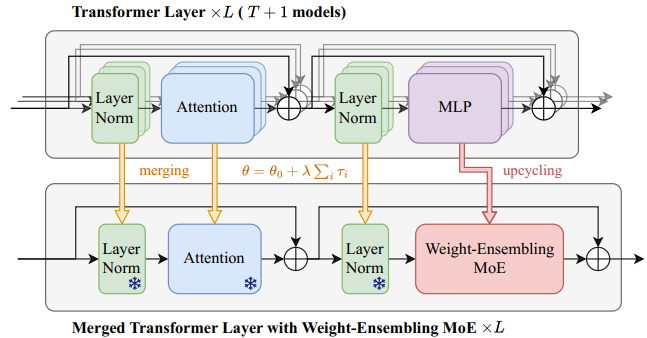
\includegraphics[width=.38\linewidth]{arch_wemoe_overview.png}
  \caption{Thiết kế WEMoE gốc trên vision Transformer chuẩn hóa trước, theo Tang và cộng sự~\cite{tang2024wemoe}. Trên: các mô hình đã tinh chỉnh và mô hình huấn luyện trước. Dưới: lớp đã hợp nhất. Các phần đóng băng có dấu bông tuyết.}
  \label{fig:overview}
\end{figure}

\begin{figure}[htbp]
  \centering
  \resizebox{.76\linewidth}{!}{\input{figures_v3_vi/architecture}}\\[2pt]
  {\scriptsize\tikz\node[frz,minimum height=.22cm,minimum width=.35cm,inner sep=0]{};~đóng băng\quad
  \tikz\node[mix,minimum height=.22cm,minimum width=.35cm,inner sep=0]{};~phụ thuộc đầu vào\quad
  \tikz\node[trn,minimum height=.22cm,minimum width=.35cm,inner sep=0]{};~huấn luyện trong FSFT}
  \caption{Mô hình WEMoE hợp nhất như đã cài đặt. Trong phạm vi full, cả fc1 và fc2 đều phụ thuộc đầu vào. Trong phạm vi intermediate-only, fc2 là tĩnh và dùng Task Arithmetic.}
  \label{fig:arch}
\end{figure}

\begin{table}[htbp]
  \centering\tablestyle
  \caption{Các thành phần của mô hình hợp nhất trong biến thể mặc định full MLP.}
  \label{tab:components}
  \begin{tabularx}{\linewidth}{l X c}
    \toprule
    Thành phần & Nguồn gốc & Trong FSFT\\
    \midrule
    Embedding, attention, chuẩn hóa lớp, pooler & Task Arithmetic với $\lambda$ chọn trên dev & Đóng băng\\
    Trọng số MLP gốc $W_0^{\ell}$ & Mô hình huấn luyện trước & Đóng băng\\
    Véc-tơ tác vụ của MLP $\tau_i^{\ell}$ & Chuyên gia trừ mô hình huấn luyện trước & Đóng băng\\
    Các head phân loại $g_t$ & Mỗi chuyên gia một head & Đóng băng\\
    Các bộ định tuyến $r^{\ell}$ & Mới, mỗi lớp encoder một bộ & \textbf{Huấn luyện}\\
    \bottomrule
  \end{tabularx}
\end{table}

Cách phân chia này quyết định chi phí lưu trữ. Phần tĩnh được lưu một lần. Mỗi lớp được nâng cấp phải giữ trọng số huấn luyện trước và một véc-tơ tác vụ cho mỗi chuyên gia, tức là $T+1$ bản của lớp đó, và các bộ định tuyến thêm tham số $\phi$ của riêng chúng:
\begin{equation}
|\theta_{\mathrm{static}}|+(T+1)\,|\theta_{\mathrm{MLP}}|+|\phi|+|\mathrm{heads}|,
\label{eq:storage}
\end{equation}
trong đó $\theta_{\mathrm{MLP}}$ là các lớp được nâng cấp. Chúng tôi đánh giá hai phạm vi: \emph{full}, nâng cấp fc1 và fc2, và \emph{intermediate-only}, chỉ nâng cấp fc1. Các véc-tơ tác vụ chiếm phần lớn tham số lưu trữ của phạm vi full (Bảng~\ref{tab:storage}), nên mức tiết kiệm phụ thuộc mạnh vào lựa chọn này. Tang và cộng sự chọn MLP dựa trên quan sát trên các mô hình CLIP-ViT rằng trọng số attention giữ hướng gần với mô hình huấn luyện trước hơn trọng số MLP. Chúng tôi không lặp lại phép đo đó trên BERT, nên lựa chọn này là kế thừa chứ chưa được kiểm chứng độc lập ở đây.

\section{Task Arithmetic và véc-tơ tác vụ}
\label{sec:ta}

Véc-tơ tác vụ (Phương trình~\ref{eq:task-vector}) ghi lại những gì tinh chỉnh đã thay đổi cho một tác vụ. Task Arithmetic~\cite{ilharco2023task} cộng các véc-tơ này vào mô hình gốc với một hệ số tỉ lệ $\lambda$:
\begin{equation}
\theta=\theta_0+\lambda\sum_{i=1}^{T}\tau_i .
\label{eq:ta}
\end{equation}
Simple Averaging là trường hợp đặc biệt $\lambda=1/T$, bằng trung bình trọng số của các chuyên gia. $\lambda$ nhỏ giữ mô hình gần mô hình huấn luyện trước, còn $\lambda$ lớn áp dụng các cập nhật mạnh hơn, kể cả những xung đột giữa chúng. Chúng tôi chọn $\lambda$ bằng tìm kiếm lưới theo điểm dev trung bình (Mục~\ref{sec:merging}). Phương pháp này đơn giản và không thêm tham số, nhưng kết quả giống nhau với mọi đầu vào.

\section{Bộ định tuyến và MLP phụ thuộc đầu vào}
\label{sec:router}

Mỗi lớp encoder có bộ định tuyến riêng $r^{\ell}$ (Hình~\ref{fig:router}). Đầu vào của nó là chuỗi trạng thái token $h^{\ell}_j\in\mathbb{R}^{d}$ ra khỏi Add\&Norm thứ nhất của lớp đó. Bộ định tuyến có hai lớp tuyến tính với ReLU và được áp dụng cho từng token:
\begin{equation}
r^{\ell}(h)=A^{\ell}_2\,\mathrm{ReLU}\big(A^{\ell}_1h+c^{\ell}_1\big)+c^{\ell}_2,
\label{eq:router}
\end{equation}
với $A^{\ell}_1\in\mathbb{R}^{d\times d}$ và $A^{\ell}_2\in\mathbb{R}^{T\times d}$. Mười hai bộ định tuyến có $12\,(d^2+d+Td+T)=7\,133\,244$ tham số huấn luyện được. Đầu ra theo token được lấy trung bình trên các vị trí không phải padding, dùng mặt nạ attention $m_j\in\{0,1\}$, để có một véc-tơ cho mỗi đầu vào, nên padding không ảnh hưởng đến định tuyến:
\begin{equation}
w^{\ell}(x)=\frac{\sum_j m_j\,r^{\ell}(h^{\ell}_j)}{\sum_j m_j}\in\mathbb{R}^{T}.
\label{eq:gating}
\end{equation}
Với đầu vào $x$, mỗi lớp tuyến tính được nâng cấp được dựng lại từ trọng số huấn luyện trước và phần tương ứng của các véc-tơ tác vụ, và bias cũng được dựng lại theo cách tương tự:
\begin{equation}
W^{\ell}(x)=W_0^{\ell}+\sum_{i=1}^{T}w_i^{\ell}(x)\,\tau_i^{\ell},\qquad
b^{\ell}(x)=b_0^{\ell}+\sum_{i=1}^{T}w_i^{\ell}(x)\,\tau_i^{\ell,b}.
\label{eq:we}
\end{equation}
Hai lớp tuyến tính của một khối dùng chung $w^{\ell}(x)$. Dự đoán dùng head $g_t$ của tác vụ đã biết, trong đó $\bar\theta$ là các trọng số hợp nhất tĩnh:
\begin{equation}
p(y\mid x,t)=\mathrm{softmax}\Big(g_t\big(\mathrm{pool}(\mathrm{BERT}(x;\bar\theta,\{W^{\ell}(x)\}))\big)\Big),\quad
\hat y=\arg\max_{y}\,p(y\mid x,t).
\label{eq:prediction}
\end{equation}

\begin{figure}[htbp]
  \centering
  \begin{minipage}[c]{.25\linewidth}\centering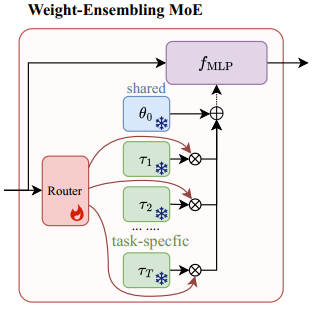
\includegraphics[width=\linewidth]{arch_wemoe_module.png}\end{minipage}\hfill
  \begin{minipage}[c]{.72\linewidth}\centering\resizebox{\linewidth}{!}{\input{figures_vi/router}}\end{minipage}
  \caption{Trái: mô-đun WEMoE của Tang và cộng sự~\cite{tang2024wemoe}. Phải: bộ định tuyến của lớp $\ell$ như đã cài đặt, áp dụng cho từng token và lấy trung bình trên các token không phải padding.}
  \label{fig:router}
\end{figure}

Các giá trị của bộ định tuyến \emph{không được chuẩn hóa}. Không có softmax và không chọn top-$k$, nên một giá trị có thể lớn hơn 1 hoặc âm, tức là bộ định tuyến có thể khuếch đại hoặc trừ đi một véc-tơ tác vụ, và phép kết hợp không lồi cũng không thưa. Trọng số tuyến tính được khởi tạo từ $\mathcal{N}(0,0.01^2)$ với $c^{\ell}_1=0$ và $c^{\ell}_2=\lambda$, nên $w^{\ell}_i(x)\approx\lambda$ lúc bắt đầu và mô hình xuất phát gần Task Arithmetic. Các unit test trên mô hình ngẫu nhiên nhỏ xác nhận rằng định tuyến hằng bằng Task Arithmetic, padding không ảnh hưởng đến định tuyến và chỉ các bộ định tuyến nhận gradient.

\section{Hàm mục tiêu Few-Shot Fine-Tuning (FSFT)}
\label{sec:fsft}

Các bộ định tuyến được huấn luyện bằng Few-Shot Fine-Tuning: cross-entropy trên một tập nhỏ có nhãn, cộng qua các tác vụ. Với mỗi tác vụ, $k$ mẫu $D_t^{(k)}$ được lấy từ một tập dự trữ, và với seed cố định thì $k$ nhỏ hơn cho một tập con của $k$ lớn hơn. Ở mỗi bước, một mini-batch $B_t$ được lấy cho mỗi tác vụ, và hàm mục tiêu là
\begin{equation}
\min_{\phi}\ \sum_{t=1}^{T}\ \frac{1}{|B_t|}\sum_{(x,y)\in B_t}-\log p_{\phi}(y\mid x,t),
\qquad B_t\subset D_t^{(k)},\ \ |D_t^{(k)}|=k ,
\label{eq:fsft}
\end{equation}
trong đó $p_\phi$ là phân phối của Phương trình~\eqref{eq:prediction}. Mọi thành phần ngoài $\phi$ được giữ đóng băng, và dropout bị tắt. Điểm dev trung bình được đánh giá trước khi huấn luyện và sau mỗi 50 bước, và trạng thái bộ định tuyến ở bước tốt nhất được khôi phục khi kết thúc. Vì vậy, một lần chạy có bước tốt nhất bằng 0 sẽ báo cáo bộ định tuyến chưa huấn luyện.

Bảng~\ref{tab:comparison} phân biệt phương pháp gốc với nghiên cứu này. Khác biệt lớn nhất là hàm mục tiêu. Tang và cộng sự tối thiểu hóa entropy của dự đoán trên dữ liệu kiểm thử không nhãn, tức là thích ứng lúc kiểm thử (test-time adaptation), và hàm mục tiêu này không được dùng ở đây. FSFT dùng các mẫu huấn luyện có nhãn và không bao giờ chạm vào tập dùng để báo cáo. Do đó, kết quả của hai nghiên cứu không so sánh trực tiếp được.

\begin{table}[htbp]
  \centering\tablestyle
  \caption{Nghiên cứu WEMoE gốc của Tang và cộng sự~\cite{tang2024wemoe} và nghiên cứu này.}
  \label{tab:comparison}
  \begin{tabularx}{\linewidth}{>{\bfseries\raggedright\arraybackslash}p{3.1cm} *{2}{>{\raggedright\arraybackslash}X}}
    \toprule
    Khía cạnh & Tang và cộng sự & Nghiên cứu này\\
    \midrule
    Backbone, tác vụ & Các mô hình thị giác CLIP-ViT; tám tác vụ phân loại ảnh & BERT-base; năm tác vụ nhị phân của GLUE\\
    Huấn luyện bộ định tuyến & Thích ứng lúc kiểm thử: entropy trên dữ liệu kiểm thử không nhãn & FSFT: cross-entropy trên $k$ mẫu có nhãn mỗi tác vụ\\
    Đầu vào định tuyến & Trung bình trên các token & Trung bình trên các token không phải padding\\
    Mô-đun được nâng cấp & Các MLP của Transformer & Full MLP; intermediate-only là ablation\\
    \bottomrule
  \end{tabularx}
\end{table}
